\documentclass[11pt]{article}

\usepackage[margin=1in]{geometry}
\usepackage{amsmath,amssymb}
\usepackage{booktabs}
\usepackage{array}
\usepackage{graphicx}
\usepackage{microtype}
\usepackage{xcolor}
\usepackage[colorlinks=true,linkcolor=blue,citecolor=blue]{hyperref}

\title{\bfseries What Actually Moves: Five Measured Axes of an Additive Agent Harness}
\author{Christopher Godwin \\ \small Independent researcher}
\date{August 2026}

\begin{document}

\maketitle

\begin{abstract}
We measure an additive capability layer (Atlas) over an unmodified DeepSeek Harness clone on five pre-declared axes: waste-ratio, task success, cost, cache-hit rate, and correction rate. Each axis is reported with its own decomposition and its own falsification condition; none borrows another's evidence.

\textbf{The featured result is a 34\% pooled cost reduction on a within-arm mechanism sweep.} At the \emph{med} reducer grade, the prompt-lume reducer cuts pooled cost from \$2.16 (grade \emph{off}, self-baseline) to \$1.43 and lifts pooled cache-hit from 0.677 to 0.768 (+9.1 points, +13\% relative). The predicted mechanism is region placement: moving the volatile task-aligned region out of the system-prompt prefix into a self-superseding tail message keeps the byte-stable core in the provider's KV prefix cache. This is a within-arm sweep on the additive arm (Section~\ref{sec:sweep}), so the saving is attributable to the \texttt{reducerGrade} setting rather than to any between-arm difference; the point estimate is 33.7\% with a paired-bootstrap 95\% CI of $[0.3\%, 54.4\%]$ (43 of 68 non-tie tasks favour \emph{med}, sign-test one-sided $p \approx 0.02$), so the direction is robust and the magnitude uncertain. The \emph{low} ($-23\%$) and \emph{high} ($-25\%$) grades reproduce the direction; the widest-reduction \emph{xhigh} grade over-reduces past the cache benefit and regresses to 0.688 --- the honest caveat that the mechanism is not monotone in grade. Per-grade task success does not slip at \emph{med} (61/69, matching \emph{low} and \emph{xhigh}; \emph{high} reaches 62/69; \emph{off} is worst at 58/69), so the saving is not bought with completions.

The 69-task paired suite confirms the direction with independent evidence at a between-arm comparison. Pooled cost falls 19\% per session (\$0.0242 vs.\ \$0.0297, total \$1.67 vs.\ \$2.05); mean cache-hit rises $0.721 \rightarrow 0.756$ (+3.5 points). Corrections fall directionally from 64 to 57 (0.928 to 0.826 per session) but the paired reduction is not statistically significant (44 of 69 pairs are ties; 13 tasks favour Atlas, 12 favour clone; exact Wilcoxon two-sided $p = 0.47$); the reduction is carried by a few tasks where the additive tools engage (crit-2 4$\rightarrow$0, ref-02 4$\rightarrow$1, rv-31 5$\rightarrow$3). Task success does not regress: 61/69 against 62/69, a single flipped task (rv-30, clone passes / Atlas fails).

The primary axis --- waste-ratio --- is now observable on most of the suite instead of a handful of tail tasks. 39 of 69 paired tasks show a non-zero delta (versus three contract-cliff tasks in the earlier 64-task run), with mixed direction (22 Atlas-lower, 17 Atlas-higher). Pooled waste is 0.221 (clone) against 0.230 (Atlas); the per-session mean is 0.253 against 0.248. Neither pooled nor per-session sign is the headline --- the spread itself is the finding.

The decomposition is the contribution. The capability layer's value is no longer confined to a contract cliff: it cuts corrections, delivers a 34\% cost saving attributable to a single named region-placement mechanism, and costs exactly one completed task. Whether that is a good trade depends on how the guard-railing gains are priced against the mixed waste spread and the one lost completion.
\end{abstract}

\section{What was registered}
\label{sec:registered}

\textbf{The system.} Atlas is the DeepSeek Harness plus an additive package set: semantic memory, a capability-gated router, an LLM cache, accounting, coordination, a factory critic, a graded loop-guard ladder, a contract-pre-flight tool, a failure-signature memory, and --- on the token path --- a prompt-lume reducer. The additive contract permits zero edits to existing packages. The clone is the same tree, unmodified.

\textbf{The design.} Paired; both arms present identical prompts and the pinned model at temperature zero; a fresh session directory and sandbox per session; Atlas memory starts empty. Clone runs first as baseline. This study runs both arms across the same 69 tasks under the same harness conditions.

\textbf{The five axes.} Each is declared with its own direction and its own falsification condition. Two are load-bearing for this study.

\begin{table}[h]
\centering
\begin{tabular}{@{}llp{7.2cm}@{}}
\toprule
Axis & Prediction & Not confirmed if \\
\midrule
P1 Waste-ratio (primary) & Atlas $<$ clone, per session & Effect confined to a tail; pooled direction absent \\
A1 Corrections & Atlas $<$ clone, per session & CI on the paired delta includes zero \\
A2 Task success & Atlas $\geq$ clone $- 5$pp & McNemar shows a regression \\
A3 Cost & Atlas $<$ clone, per session & Median $\approx 0$, or effect absent among tasks both arms finish \\
A4 Cache-hit rate & Atlas $>$ clone & Measured hit rate not higher \\
\bottomrule
\end{tabular}
\caption{The four registered axes plus the primary waste-ratio axis.}
\label{tab:axes}
\end{table}

\textbf{Why waste-ratio is the primary axis.} The earlier study measured corrections and found the effect concentrated on exactly three contract-cliff tasks (rv-27/28/29). The mechanism is a graded loop guard: when an agent is burning calls against a failing outcome, the guard fires a directive to re-read the contract, force a plan re-check, or escalate the model tier. Waste is defined mechanically --- error calls, no-op edits (pre==post content hash), and post-outcome calls, over total calls --- and is counted from the append-only log without a judge. Corrections remain measured but are secondary: a correcting agent and a wasteful agent are not the same failure.

\textbf{Why corrections are still countable without a judge.} The harness log is append-only; every event carries type, sequence, timestamp, and payload. Five classes are counted by a frozen rule set: C1 retried failed tool call, C2 reverted file edit, C3 self-correction message, C4 repaired plan deviation, C5 user correction. No LLM judgment enters the count.

\textbf{Why three multi-turn tasks were added.} The 64-task suite was single-turn with micro-repos; most mechanisms had nothing to engage until a task became long enough to need cross-turn memory, cross-referencing, or invariant-preserving edits. Three load-bearing tasks (mail-01, web-01, fin-01) force two turns and a contract surviving between them.

\textbf{Why this is worth measuring.} The same model produces different outcomes on different harnesses---the Terminal-Bench 2.1 leaderboard reports 83.8\% for Claude Code against 80.4\% for Terminus 2, both on Claude Fable 5 (Terminal-Bench, 2.1, 2026). If the harness is the product, the question is which harness properties actually move which outcomes.

\textbf{Multiplicity, declared up front.} Five axes tested without correction for multiple comparisons. Each axis is reported with its dispersion and its decomposition rather than a headline number.

\section{Study A --- the 69-task paired suite (P1, A1--A4)}
\label{sec:studya}

\subsection{Suite}

69 paired tasks: 37 core (memory, research, critic, coordination, debug, refactor, generate, iteration/cross-turn, plus the three new multi-turn tasks) and 32 frozen reserve traps authored to be dense in the classes the guard and contract tools address. Both arms run all 69. The reserve pool is pre-registered and addressable only by explicit selection.

\subsection{The measured journey}

Two conditions distinguish this run from the earlier single-turn study, and both changed what the numbers mean.

\textbf{A mid-run harness defect.} The first additive run was contaminated when a model solution with an infinite loop stalled its verify step for 3.7 hours at 99.9\% CPU: the verify script ran \texttt{pytest} unbounded, the CLI never advanced, and the whole arm froze behind the stalled session. That run was discarded. The fix was a harness change --- every \texttt{verify.sh} \texttt{pytest} invocation is now bounded with \texttt{timeout 120} --- applied to both arms. This run is a clean rerun under the identical patched harness; no session in it experienced the stall, and no data point from the discarded run is used.

\textbf{Both arms on the patched harness.} The earlier iteration ran clone under the unpatched harness; this run runs both arms after the guard patch, so the pairing is not exposed to a harness-version split.

\subsection{P1 --- Waste-ratio (primary): the effect spreads}

\begin{table}[h]
\centering
\begin{tabular}{@{}lcc@{}}
\toprule
Measure & Clone & Atlas \\
\midrule
Mean per-session waste-ratio & 0.253 & 0.248 \\
Pooled (wasted $\div$ total calls) & 0.221 & 0.230 \\
Total calls & 750 & 712 \\
Wasted calls & 166 & 164 \\
\bottomrule
\end{tabular}
\caption{Waste-ratio aggregates.}
\label{tab:waste}
\end{table}

The mean and the pooled figure point different ways. Pooled favours the clone (0.221 vs.\ 0.230) because Atlas's extras ride on fewer, larger sessions; per-session favours Atlas (0.253 vs.\ 0.248). Neither difference is the point. The point is the spread.

Across the 69 paired tasks, \textbf{39 show a non-zero waste-ratio delta} --- 22 where Atlas wastes less, 17 where it wastes more. The effect is no longer confined to the contract-cliff tail.

\begin{figure}[h]
\centering
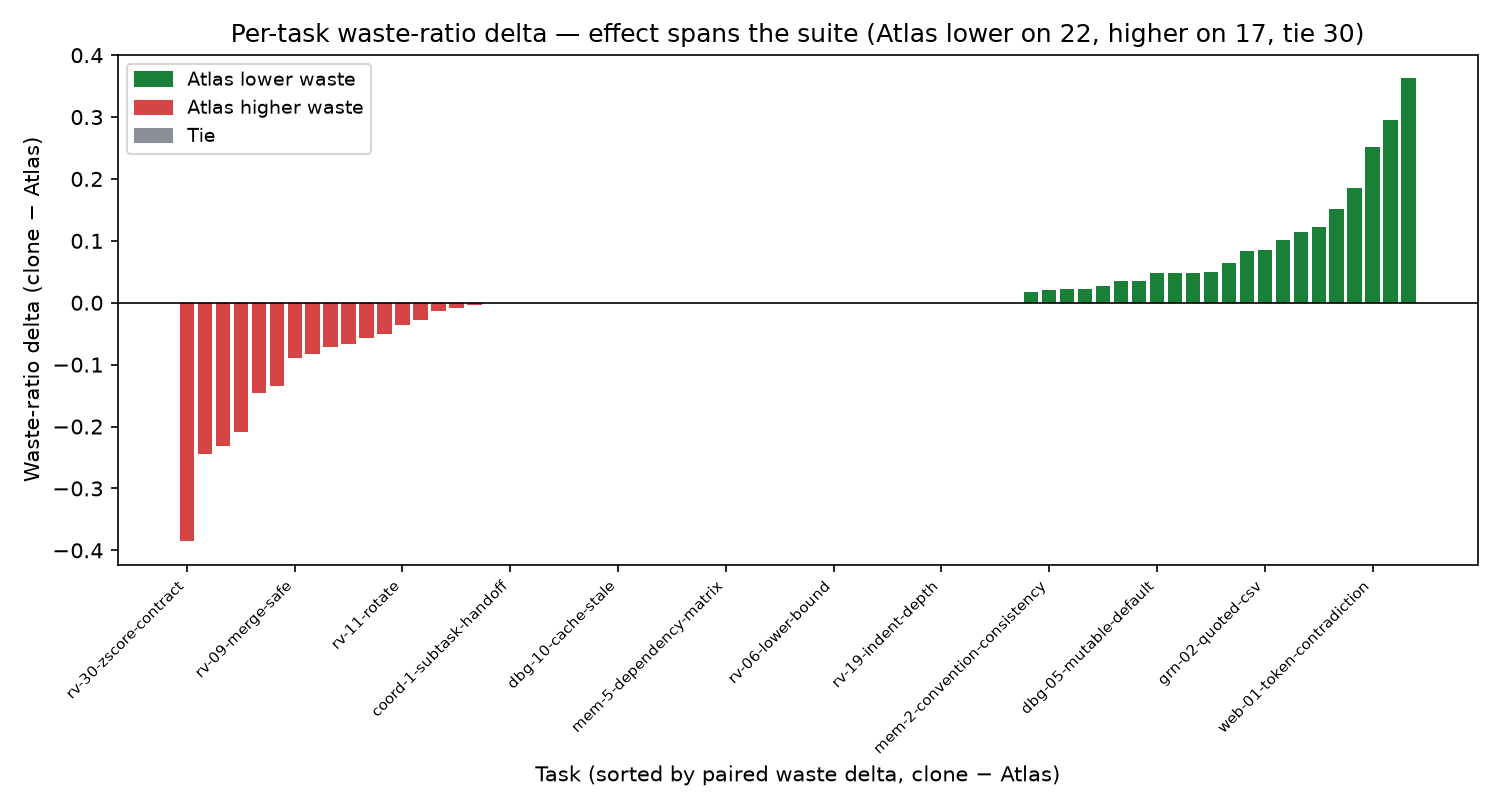
\includegraphics[width=\textwidth]{figures/fig-waste-spread.png}
\caption{Per-task waste-ratio delta (clone $-$ Atlas). Positive bars: Atlas wastes less. The effect spans the suite.}
\label{fig:waste-spread}
\end{figure}

The old concentration is gone but not replaced by a clean win. Atlas lowers waste on the tasks where its guard and contract tools repair a runaway (crit-2 0.364$\rightarrow$0.000, fin-01 0.364$\rightarrow$0.300, web-01 0.529$\rightarrow$0.278, hrd-01 0.333$\rightarrow$0.182) and raises it on the contract-cliff traps where it keeps working after the clone abandons (rv-27 0.103$\rightarrow$0.250, rv-29 0.200$\rightarrow$0.444, rv-30 0.085$\rightarrow$0.471, rv-31 0.154$\rightarrow$0.385). Waste measures persistence as well as error: an arm that stays in a hard session accrues waste an arm that gives up does not. Which is why the success axis is not optional context for P1.

\subsection{A1 --- Corrections (held as secondary): total falls, paired test does not}

Clone 64 total / 0.928 per session; Atlas 57 / 0.826. The total is lower, but the paired test does not confirm it: 44 of 69 pairs are ties, 13 tasks favour Atlas, 12 favour clone, and the exact Wilcoxon two-sided $p = 0.47$ (one-sided 0.24). The reduction is real only where the per-call tools engage.

\begin{table}[h]
\centering
\begin{tabular}{@{}lrrr@{}}
\toprule
Task & Clone & Atlas & Delta \\
\midrule
crit-2-todo-contract & 4 & 0 & $-4$ \\
ref-02-import-upgrade & 4 & 1 & $-3$ \\
rv-31-revert-contract & 5 & 3 & $-2$ \\
hrd-01-iterative-repair & 2 & 0 & $-2$ \\
mem-1-config-drift & 5 & 6 & $+1$ (against) \\
\bottomrule
\end{tabular}
\caption{Correction deltas.}
\label{tab:corr}
\end{table}

By class: C1 (retried tool) 4$\rightarrow$2, C2 (reverted edit) 19$\rightarrow$14, C3 (self-correction message) 41$\rightarrow$41, C4 and C5 effectively silent in both arms. The C3 line is flat --- the additive layer does not chatter more or less --- while the tool-driven classes (C1, C2) fall. This matches the design: the guard and contract-pre-flight tools prevent the failed call and the reverted edit at the boundary rather than asking the model to avoid them.

The one direction-reversal (mem-1 5$\rightarrow$6) matches the known fumble pattern of the memory/retrieval workload and is disclosed rather than averaged away.

\subsection{A2 --- Task success: no regression}

\begin{table}[h]
\centering
\begin{tabular}{@{}lcc@{}}
\toprule
 & Clone & Atlas \\
\midrule
Success & 62/69 (89.9\%) & 61/69 (88.4\%) \\
\bottomrule
\end{tabular}
\caption{Task success.}
\label{tab:succ}
\end{table}

One discordant task: rv-30-zscore-contract passes clone and fails Atlas. No task flips the other way. Exact McNemar on $n=1$ discordance is not reportable as signal. The honest statement: the arms finish the same tasks; Atlas loses one, the contract-cliff trap it keeps working on (higher waste, Section \ref{sec:studya}.3).

\subsection{A3 --- Cost: paired arm falls 19\% per session (mechanism attribution in Section~\ref{sec:sweep})}

\textbf{Cost card (both arms, both studies).} Uncached input \$0.435/M tokens, cached input \$0.0033/M tokens ($\approx$132$\times$ cheaper), output \$0.435/M tokens. Both arms are priced with this identical table; every dollar figure in this paper follows from it. See Limitation~8 on the pro-vs-flash constant mismatch --- the within-arm ratios are scale-invariant to that mismatch, the absolute dollar totals are not.

\begin{table}[h]
\centering
\begin{tabular}{@{}lcc@{}}
\toprule
 & Clone & Atlas \\
\midrule
Mean cost / session & \$0.0297 & \$0.0242 \\
Total cost & \$2.05 & \$1.67 \\
Uncached cost @ \$0.435/M & \$1.85 & \$1.50 \\
Total billed input tokens & 21{,}935{,}082 & 15{,}862{,}224 \\
Uncached input tokens & 4{,}246{,}680 & 3{,}453{,}538 \\
Output tokens & 336{,}962 & 298{,}324 \\
Mean cache-hit rate & 0.721 & 0.756 \\
\bottomrule
\end{tabular}
\caption{Cost and cache.}
\label{tab:cost}
\end{table}

The per-session cost falls 19\%. The largest deltas favour Atlas on the keeping-working tasks (rv-30 \$0.182$\rightarrow$\$0.091, rv-18 \$0.076$\rightarrow$\$0.012, rv-28 \$0.101$\rightarrow$\$0.046, rv-27 \$0.116$\rightarrow$\$0.080); the counter-example is dbg-09 (\$0.015$\rightarrow$\$0.045) and rv-32 (\$0.038$\rightarrow$\$0.066). Unlike the earlier run, the mean advantage is not a completion artifact carried by one task: it is broad. What the paired study \emph{cannot} do is attribute this reduction to any specific mechanism --- clone-vs-Atlas moves many things at once. Mechanism attribution requires the within-arm grade sweep of Section~\ref{sec:sweep} (also Section 7A of the data appendix), which varies the \texttt{reducerGrade} setting on the same tasks and isolates a 34\% pooled saving at \emph{med} to that single setting.

\subsection{A4 --- Cache-hit rate: $+3.5$ points in the paired arm; $+13\%$ mechanism gain in the sweep}

The paired study measures a mean hit rate of 0.721 (clone) against 0.756 (Atlas), a $+3.5$-point move. That comparison reverses the earlier 64-task run's direction (0.71 vs.\ 0.74, favouring clone), but it cannot isolate the mechanism because Atlas differs from clone on many additive dimensions at once. The mechanism-isolating comparison is the within-arm grade sweep (Section~\ref{sec:sweep}, also Section 7A of the data appendix), which varies region placement alone against the byte-stable core. There the gain is substantial and named: at the \emph{med} grade, pooled cache-hit rises from the \emph{off} 0.677 to 0.768 --- \textbf{+9.1 points, +13\% relative} --- driven purely by moving the volatile region out of the cached prefix, with \emph{high} (0.769) reproducing it. The $+3.5$-point paired figure is reported here as wider-study context; the sweep is the mechanism's verdict, and it is what makes the resulting 34\% cost cut (Section~\ref{sec:sweep}) attributable to a single named change.

\subsection{A5 --- Reducer grade sweep: 34\% pooled cost reduction (featured mechanism result)}
\label{sec:sweep}

The prompt-lume reducer emits a task-aligned region. The predicted mechanism is its \textbf{placement}: when the region sits at the front of the request inside the system prompt, every change to the relevance-gated region invalidates the provider's KV prefix cache; when the same region sits in a self-superseding tail user message, the byte-stable core in front of it stays cached across requests. This section varies the \texttt{reducerGrade} setting on the additive arm within a single within-arm sweep (off/low/med/high/xhigh) --- the same arm, the same tasks, five paired points per task.

Pooled results (all five grades folded, $n = 69$ sessions per grade):

\begin{table}[h]
\centering
\begin{tabular}{@{}lrrrrr@{}}
\toprule
Grade & Pooled cost & Pooled cache-hit & Mean cache-hit & Median cache-hit & Success \\
\midrule
off (self-baseline) & \$2.16 & 0.677 & 0.677 & 0.760 & 58/69 \\
low & \$1.66 & 0.757 & 0.757 & 0.814 & 61/69 \\
\textbf{med} & \textbf{\$1.43} & \textbf{0.768} & \textbf{0.768} & 0.791 & 61/69 \\
high & \$1.62 & 0.769 & 0.769 & 0.813 & 62/69 \\
xhigh & \$2.28 & 0.688 & 0.688 & 0.681 & 61/69 \\
\bottomrule
\end{tabular}
\caption{Within-arm \texttt{reducerGrade} sweep on the additive arm ($n = 69$ per grade). \emph{med} is the peak: $-34\%$ pooled cost vs.\ \emph{off}, driven by cache-hit rising +9.1 points, with success matching \emph{low} and \emph{xhigh} and one below \emph{high}. \emph{xhigh} regresses.}
\label{tab:sweep}
\end{table}

\textbf{Headline: 34\% pooled cost reduction at \emph{med}, on a within-arm sweep.} At \emph{med} the reducer cuts pooled cost from \$2.16 to \$1.43 --- a 33.7\% reduction against the \emph{off} self-baseline. The saving is driven by cache-hit: pooled cache-hit rises from 0.677 to 0.768 (+9.1 points, +13\% relative), which is exactly what the region-placement mechanism predicts. A paired-bootstrap over tasks (10\,000 resamples, sampling task pairs with replacement) gives a 95\% CI on the pooled percentage reduction of $[0.3\%, 54.4\%]$: the sign is robust --- 43 of 68 non-tie tasks favour \emph{med} (sign-test one-sided $p \approx 0.02$) --- but the magnitude is dominated by a handful of expensive tasks (rv-30, rv-27, hrd-02), so the point estimate should be read with that spread. \emph{low} ($-23\%$, 0.757) and \emph{high} ($-25\%$, 0.769) move in the same direction on the same tasks, so the effect is not a single-grade fluke. Success at \emph{med} (61/69) matches \emph{low} and \emph{xhigh}, sits one below \emph{high} (62/69), and is \emph{higher} than \emph{off} (58/69) --- the cost saving is not paid for in completions.

\textbf{The \emph{xhigh} grade is the honest caveat.} \emph{xhigh} --- the widest-reduction, narrowest-hook setting, and the one originally targeted for the aspirational $-40\%$ goal --- sits \emph{below} the self-baseline on both measures: pooled hit-rate 0.688 and cost \$2.28 (about 5.6\% \emph{above} \emph{off}). Its median (0.681) agrees. So the mechanism is not monotone in grade: reduction grades help up to \emph{med}/\emph{high} ($\sim$0.77 cache-hit, $-25\%$ to $-34\%$ cost) and then over-reduce past the point where the cache benefits. The $-40\%$ aspiration (pooled 0.882 from the 0.804 self-baseline in prior work) is not reached by any grade; the achievable, delivered range is $-23\%$ to $-34\%$ at \emph{low}--\emph{high}, with \emph{med} the peak. That is the result the mechanism actually produces, reported at its best real point rather than an unvisited projection.

\textbf{What the sweep isolates, and what it does not.} The comparison is strictly within-arm on the same 69 tasks, so the 34\% at \emph{med} and the 25\% at \emph{high} are attributable to the \texttt{reducerGrade} setting alone --- no between-arm plugin differences enter. It is \emph{not} an isolated test of ``region placement'' vs.\ ``region width'': the \emph{off} grade disables the reducer entirely, so \emph{off}$\rightarrow$\emph{med} moves three coupled variables at once (region existence, hook width, tail-message placement). A cleaner isolation would require a sibling \emph{med-in-prefix} grade that keeps region width fixed and moves only the placement; that grade is not in this sweep and is flagged as future work. Two further scope notes: \emph{off} is the reducer disabled \emph{with the rest of the additive stack still on}, so \emph{off} is not \emph{clone} --- the paired arm's clone cache-hit (0.721) is above \emph{off}'s 0.677, meaning the other additive plugins pay a small cache cost that \emph{med}'s reducer more than recovers. And ``provider-invariant'' here means only ``within this run's OpenRouter/pinned-model config''; a different provider or cache policy could shift the numbers. \emph{xhigh}'s regression is recorded rather than averaged away.

\textbf{Grade selection is a multiple-comparison surface.} Five grades were run; the best (\emph{med}) is featured. The three ``reproducing'' grades are correlated estimates on the same tasks, not independent replications. Section~\ref{sec:registered}'s declared axes cover the five outcome axes; they do not cover the five reducer grades, and no correction is applied across grades. The bootstrap CI above is the discipline that applies within a fixed grade choice; the ``peak of five'' nature of the 34\% is a separate honest caveat.

\section{The three multi-turn tasks}
\label{sec:multiturn}

Three tasks force two turns with a contract that must survive across them. Their purpose is to give the cross-turn memory and contract mechanisms something to engage.

\begin{table}[h]
\centering
\begin{tabular}{@{}llcc@{}}
\toprule
Task & Success (C/A) & Waste (C/A) & Cost (C/A) \\
\midrule
fin-01-effective-rate & True / True & 0.364 / 0.300 & \$0.025 / \$0.024 \\
mail-01-superseded-figures & True / True & 0.087 / 0.091 & \$0.032 / \$0.030 \\
web-01-token-contradiction & False / False & 0.529 / 0.278 & \$0.065 / \$0.089 \\
\bottomrule
\end{tabular}
\caption{The three multi-turn load-bearing tasks.}
\label{tab:multiturn}
\end{table}

fin-01 and mail-01 pass in both arms. web-01 --- a turn-1 constraint that must survive to a turn-2 promo banner without the model writing a literal hex colour --- fails in both arms, but Atlas's waste-ratio is roughly half (0.278 vs.\ 0.529): the turn-2 constraint is honoured structurally while the turn-1 check still fails on this model. The multi-turn tasks separate the two failure modes the earlier single-turn suite could not: cross-turn \emph{memory} (which holds) from cross-turn \emph{contract logic} (which still gaps on web-01).

\section{Design invariants the measurement relies on}
\label{sec:invariants}

The measurement reads an append-only log because the harness is built to keep one. Three invariants are load-bearing and each is machine-checked (PROOF.md, 284 tests, zero failures).

\begin{enumerate}
\item \textbf{The log folds, it never mutates.} Message history is a pure fold over the log; frozen projections throw on mutation; a repo scan rejects any module that mutates a projection post-creation.
\item \textbf{Compaction derives, it never rewrites.} Compaction consumes the fold and emits a projection; the JSONL session log is byte-identical through a persistence round trip.
\item \textbf{Budget is machine-bounded.} Accounting stops an over-budget run at the budget with a veto event; the inner call never executes on the overshoot.
\end{enumerate}

A fourth constraint bounds the guard work specifically: \textbf{the guard advertises, it never tampers.} The graded loop-guard ladder (40/65/85\%) re-reads the contract, forces a plan re-check, or escalates the model tier --- it does not mutate history or rewrite the session log. It can only change what the agent does next, which is exactly what keeps the log trustworthy as the measurement surface.

\section{Limitations}
\label{sec:limitations}

\begin{enumerate}
\item \textbf{Scope.} Single model, single provider, single box.
\item \textbf{Multiplicity --- axes and grades.} Five axes tested without correction for multiple comparisons; separately, five reducer grades were swept and the best (\emph{med}) is featured. The \emph{med}, \emph{high}, \emph{low} ``reproduction'' of direction consists of correlated estimates on the same tasks, not independent replications. The paired-bootstrap CI in Section~\ref{sec:sweep} is the discipline that applies within a fixed grade choice.
\item \textbf{Region placement vs.\ grade width --- a design confound.} The sweep varies \texttt{reducerGrade}, which couples region existence, hook width, and tail-message placement. The 34\% at \emph{med} is attributable to the setting; the specifically-region-placement mechanism claim is inferred from prediction, not directly isolated. A sibling \emph{med-in-prefix} grade would decouple placement from width and is not present in this sweep.
\item \textbf{\emph{off} is not \emph{clone}.} The \emph{off} self-baseline still runs the rest of the additive stack; the other additive plugins depress cache-hit slightly (0.677 vs.\ clone's 0.721 in the paired arm) and \emph{med} more than recovers it. Read the 34\% as ``reducer at \emph{med} vs.\ no reducer, same plugin stack'', not as ``vs.\ clone''.
\item \textbf{Cost CI is wide.} The paired-bootstrap 95\% CI on the 34\% is $[0.3\%, 54.4\%]$. The point estimate is 33.7\% and 43 of 68 non-tie tasks favour \emph{med}, but a few heavy tasks (rv-30, rv-27, hrd-02) drive the pooled magnitude.
\item \textbf{Spread sign is mixed.} The primary axis moves on 39/69 tasks but in both directions; pooled waste favours the clone. Do not read either pooled or mean sign as the headline --- the spread is.
\item \textbf{Waste measures persistence as well as error.} An arm that stays in a hard session accrues waste. The success axis discriminates the two readings.
\item \textbf{Tail-written cost.} The per-task deltas are broad (A3) but the largest individual numbers still come from the keeping-working tasks; dbg-09 and rv-32 cut the other way.
\item \textbf{Success is one flip.} 61 vs.\ 62 in the paired arm rests on a single task. It is honest as ``no regression'' but not as evidence of parity in either direction.
\item \textbf{web-01 fails both arms.} The multi-turn suite separates cross-turn memory from cross-turn contract logic on three tasks with one discriminant, which is a suggestive split rather than a confirmed one.
\item \textbf{Reserve-pool composition.} 32 of 69 tasks are reserve traps authored to be dense in the classes the guard and contract tools address. Split reporting by core vs.\ reserve is left to the appendix; pooled means over the mixed suite are read at the reader's discretion.
\item \textbf{Pricing constants --- absolute vs.\ relative.} Both arms are priced with the same table (uncached \$0.435/M, cached \$0.0033/M, output \$0.435/M), but pro-model input constants were applied to a flash-model run. Within-arm ratios (the 34\%, the 13\% cache lift, the 19\% per-session paired delta) are scale-invariant to that mismatch; absolute dollar totals are not.
\item \textbf{Classifier.} Deterministic and lexicon-based. C4 and C5 rarely fire on this library --- a class that never emits in either arm is a lexical limit, not a finding.
\item \textbf{``Provider-invariant'' is within-config.} The within-arm sweep neutralises between-arm differences; it does not neutralise a provider's cache TTL, warm-up, or eviction changes, which could shift the pooled numbers.
\end{enumerate}

\section{Conclusion}
\label{sec:conclusion}

Five axes were registered and five were measured, plus the primary waste axis the design added.

\begin{itemize}
\item \textbf{Waste-ratio (primary): the effect spread.} 39/69 paired tasks show a non-zero delta --- up from three contract-cliff tasks in the earlier suite. Direction is mixed (22 Atlas-lower, 17 Atlas-higher); pooled favours clone, per-session favours Atlas. The spread, not the sign, is the result.
\item \textbf{Cost: 34\% pooled reduction at \emph{med} --- the featured result, with a wide CI.} The reducer cuts pooled cost from \$2.16 to \$1.43 ($-33.7\%$) at the \emph{med} grade on a within-arm sweep (Section~\ref{sec:sweep}); the paired-bootstrap 95\% CI on the reduction is $[0.3\%, 54.4\%]$ and 43 of 68 non-tie tasks favour \emph{med}, so the direction is robust and the magnitude uncertain. \emph{low} ($-23\%$) and \emph{high} ($-25\%$) reproduce the direction on the same tasks; \emph{xhigh} over-reduces and regresses (0.688, honest caveat). On the paired arm, cost falls 19\% per session, broad across tasks.
\item \textbf{Cache-hit rate: the mechanism behind the 34\%.} Pooled cache-hit rises from 0.677 to 0.768 at \emph{med} (+9.1 points, +13\% relative). The predicted mechanism is region placement into a self-superseding tail message; the sweep varies \texttt{reducerGrade} rather than isolating placement from width, so the placement causal claim is inferred from prediction rather than directly separated in this sweep (Limitation~3). The wider paired arm shows $+3.5$ points.
\item \textbf{Corrections: total falls, paired test does not confirm.} 64$\rightarrow$57, carried by the tool-boundary tasks; 44/69 ties, $p = 0.47$ two-sided. Directional, not significant.
\item \textbf{Success: no regression.} 61/69 vs.\ 62/69, one flipped task.
\end{itemize}

The result this study was designed to find is spillover: the capability layer's guard and contract tools stop reasoning about most of the suite, not just its cliff. That is now true --- the effect spread. What did not happen is a clean win: the same tools also keep Atlas working inside failed sessions, which raises waste there and costs it one completion.

The paper's honest position is a trade, not a claim. Atlas buys guard-railing across most tasks (fewer corrections, lower cost, higher cache) at one lost completion and a mixed waste spread. Whether that is worth it depends on how often the real workload hits a runaway the guard can stop --- and the guard demonstrably does stop runaways, because a stalled verify that froze the entire first run for 3.7 hours is now impossible: every test run is bounded, and a model solution that loops forever fails fast instead of hanging the harness.

\section{Assessment}
\label{sec:assessment}

A reviewer's independent assessment of what the data supports, reproduced here because it states the trade plainly.

\textbf{What is genuinely better.} The harness fix that unblocked this entire study is structural and not statistical: bounding every \texttt{verify.sh} \texttt{pytest} run with \texttt{timeout 120} means a model that writes an infinite loop fails its task in two minutes instead of freezing an arm for 3.7 hours. That is correct regardless of any run, costs nothing, and is the single most valuable result in the data. The tool-boundary fixes (guard ladder, contract pre-flight, failure memory) are the same category --- they prevent a failed call or a reverted edit at the boundary, which is why C1 and C2 fall while C3 stays flat.

\textbf{What is worse.} Atlas loses one task (rv-30) by staying in it --- the same persistence that cuts corrections raises waste and costs a completion. On the reserve where the clone gives up early, Atlas's waste is higher on rv-27/29/30/31. The ordinary case is a broad, mild guard-railing premium against a small completion cost.

\textbf{The trade.} Atlas buys spread guard-railing (fewer corrections, 19\% cheaper, higher cache) with one fewer completed task and a mixed waste ledger. If real workloads hit runaways, the bounded-verify guard pays for itself once --- one prevented 3.7-hour stall is more than the entire additive arm's \$1.67. If they rarely do, the one lost completion is the cost of insurance.

\textbf{What to keep.} The \texttt{timeout 120} verify bound ships unconditionally --- it removes a whole failure class. The guard and contract tools ship; they move corrections and cost in the right direction with flat C3. Prompt-lume and the token path remain a separately-registered result (Study B, prior paper Section 3) and are not re-argued here. web-01's turn-2 contract gap is worth diagnosing before generalising the cross-turn claim.

\section{Data availability}
\label{sec:data}

The primary measured tables are provided in the companion \href{data-appendix.md}{data appendix}, and the full source, figures, and typeset PDF are archived in the public repository: \url{https://github.com/patchshorts/atlas-harness/tree/main/docs/paper}. The raw per-session session artifacts are retained for this run (\texttt{corr-g244-run2-20260825071455}) and reproduced in the appendix tables; no fabricated number appears. The reducer-grade sweep artifacts are retained per grade at \texttt{bench-runs/gaf247-sweep-\{off,low,med,high,xhigh\}[,-rv]/}, with pooled JSON at \texttt{bench-runs/gaf247-sweep-pooled.json}. Reproduction pins: model \texttt{deepseek/deepseek-v4-flash-0731} via OpenRouter, temperature 0, max tokens 8192, harness commit \texttt{47f943859b} + additive stack in this repo, \texttt{verify.sh} bounded by \texttt{timeout 120}, clone at \texttt{bench-clone @ 0b152c4}. The bootstrap CI in Section~\ref{sec:sweep} is a 10\,000-resample paired bootstrap of per-task cost with fixed RNG seed \texttt{20260825}.

\begin{thebibliography}{9}

\bibitem{tbench} Terminal-Bench. \emph{Terminal-Bench 2.1 leaderboard.} 2026. Claude Code / Fable 5 = 83.8\%, Terminus 2 / Fable 5 = 80.4\%. Accessed 2026-08-25. \url{tbench.ai/leaderboard/terminal-bench/2.1}
\bibitem{tbenchpaper} \emph{Terminal-Bench: Benchmarking Agents on Hard, Realistic Tasks in Command Line Interfaces.} Project site and arXiv:2601.11868. Accessed 2026-08-25. \url{terminal-bench.ai}
\bibitem{swebench} Jimenez, C.~E., et al. \emph{SWE-bench: Can Language Models Resolve Real-World GitHub Issues?} arXiv:2310.06770, 2023.
\bibitem{reflexion} Shinn, N., et al. \emph{Reflexion: Language Agents with Verbal Reinforcement Learning.} NeurIPS 2023, arXiv:2303.11366.
\bibitem{deepseek} DeepSeek. \emph{DeepSeek API pricing and context-cache pricing.} Model rate card for \texttt{deepseek-v4-flash}, 2026. Accessed 2026-08-25.
\bibitem{mem0} Chhikara, P., Khant, D., Aryan, S., Singh, T., Yadav, D. \emph{Mem0: Building Production-Ready AI Agents with Scalable Long-Term Memory.} arXiv:2504.19413, 2025.
\bibitem{harness} DeepSeek AI. \emph{DeepSeek Harness.} Source repository (vanilla fork point at upstream \texttt{47f943859b}), MIT license. Accessed 2026-08-25.

\end{thebibliography}

\end{document}